\tikzstyle{input_neuron}=[circle,draw=red!50,fill=red!10,thick,minimum size=6mm]
\tikzstyle{hidden_neuron}=[circle,draw=blue!50,fill=cyan!10,thick,minimum size=6mm]
\tikzstyle{output_neuron}=[circle,draw=green!50,fill=green!10,thick,minimum size=6mm]
\tikzstyle{extra_dots} = [circle,draw = black,fill=black!100,thick,minimum size=0.001mm,size=0.01cm]
\tikzstyle{input}=[circle,draw=black!50,fill=black!20,thick,minimum size=6mm]

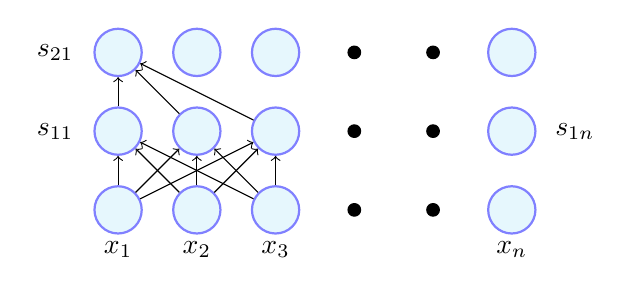
\begin{tikzpicture}

	\node [hidden_neuron] (neuron11) at (3.5,7.5) {} ;
	\node(text1) at(3.5,7){$x_1$};
	\node [hidden_neuron] (neuron12) at (4.5,7.5) {} ;
	\node(text1) at(4.5,7){$x_2$};
	\node [hidden_neuron] (neuron13) at (5.5,7.5) {} ;
	\node(text1) at(5.5,7){$x_3$};

	\node(text) at (9.3,8.5){$s_{1n}$};
	\node(text) at (2.7,8.5){$s_{11}$};
	\node(text) at (2.7,9.5){$s_{21}$};
	\node [hidden_neuron] (neuron14) at (8.5,7.5) {} ; 
	\node(text1) at(8.5,7){$x_n$};
	\node [hidden_neuron] (neuron21) at (3.5,8.5) {} ;
	\node [hidden_neuron] (neuron22) at (4.5,8.5)  {};
	\node [hidden_neuron] (neuron23) at (5.5,8.5)  {};
	\node [hidden_neuron] (neuron31) at (3.5,9.5)  {};
	\node [hidden_neuron] (neuron32) at (4.5,9.5) {} ;
	\node [hidden_neuron] (neuron33) at (5.5,9.5)  {};

	%\node [extra_dots] (dot3) at (6.5,8.5)  ;
	\draw [black,fill=black](6.5,8.5)circle (0.8mm);
	\draw [black,fill=black](7.5,8.5)circle (0.8mm);
	\draw [black,fill=black](6.5,7.5)circle (0.8mm);
	\draw [black,fill=black](7.5,7.5)circle (0.8mm);

	\draw [black,fill=black](6.5,9.5)circle (0.8mm);
	\draw [black,fill=black](7.5,9.5)circle (0.8mm);


	%\node [extra_dots] (dot4) at (7.5,8.5)  ;
	\node [hidden_neuron] (neuron24) at (8.5,8.5) {} ; 
	\node [hidden_neuron] (neuron34) at (8.5,9.5) {} ; 
	\draw[->](neuron11)--(neuron21);
	\draw[->](neuron12)--(neuron21);
	\draw[->](neuron13)--(neuron21);
	\draw[->](neuron11)--(neuron22);
	\draw[->](neuron12)--(neuron22);
	\draw[->](neuron13)--(neuron22);

	\draw[->](neuron11)--(neuron23);
	\draw[->](neuron12)--(neuron23);
	\draw[->](neuron13)--(neuron23);

	\draw[->](neuron21)--(neuron31);
	\draw[->](neuron22)--(neuron31);
	\draw[->](neuron23)--(neuron31);

\end{tikzpicture}